\newpage
\section{Design pattern utilizzati}
Nella progettazione di \glossaryItem{MaaS} sono stati utilizzati i seguenti \textit{design pattern}:
\begin{itemize}
\item \textbf{Builder};
\item \textbf{Facade};
\item \textbf{Singleton};
\item \textbf{Chain of Responsibility};
\item \textbf{Model-View-Controller}.
\end{itemize}
Verrà presentata una descrizione di questi \textit{design pattern}, dividendoli in base al loro tipo, ovvero:
\begin{itemize}
\item \textbf{Creazionali}: Builder e Singleton;
\item \textbf{Strutturali}: Facade;
\item \textbf{Comportamentali}: Chain of responsibility;
\item \textbf{Architetturali}: Model-View-Controller.
\end{itemize}
Nella descrizione dell'architettura sono stati evidenziati i punti di applicazione dei singoli \textit{design pattern}. In questa sezione vengono riportati solamente i componenti che li realizzano nel concreto o, ove risultasse più chiaro, il \glossaryItem{diagramma delle classi} vero e proprio.
\subsection{Creazionali}
\subsubsection{Builder}
\paragraph{Descrizione} \mbox{} \\
Il \textit{design pattern} Builder separa la costruzione di un oggetto complesso dalla sua rappresentazione cosicché il \glossaryItem{processo} di costruzione stesso possa creare diverse rappresentazioni. L'algoritmo per la creazione di un oggetto complesso è indipendente dalle varie parti che costituiscono l'oggetto e da come vengono assemblate. \\
Ciò ha l'effetto immediato di rendere più semplice la classe, permettendo a una classe \textit{Builder} separata di focalizzarsi sulla corretta costruzione di un'istanza e lasciando che la classe originale si concentri sul funzionamento degli oggetti. Questo è particolarmente utile quando si vuole assicurare che un oggetto sia valido prima di istanziarlo, e non si vuole che la logica di controllo appaia nei costruttori degli oggetti. Un builder permette anche di costruire un oggetto passo-passo, cosa che si può verificare quando si fa il parsing di un testo o si ottengono i parametri da un'interfaccia interattiva. \\
A differenza dei \textit{design pattern} \textit{Abstract Factory} e \textit{Factory Method}, il cui scopo è permettere il polimorfismo, l'intenzione del \textit{Builder} è quella di ridurre il cosiddetto \textit{effetto telescoping} nei costruttori, che porta ad un grande numero di parametri richiesti in \glossaryItem{fase} di costruzione dell'oggetto.
\paragraph{Vantaggi} \mbox{} \\
\begin{itemize}
\item Permette di variare la rappresentazione interna di un oggetto;
\item Incapsula il codice della costruzione;
\item Fornisce maggiore controllo sui passi di costruzione dell'oggetto;
\end{itemize}
\paragraph{Svantaggi} \mbox{} \\
\begin{itemize}
\item Richiede la creazione di un oggetto separato (\textit{ConcreteBuilder}) per ogni tipo di oggetto da costruire (\textit{Product}).
\end{itemize}
\paragraph{Struttura}
\begin{figure}[H]
\centering
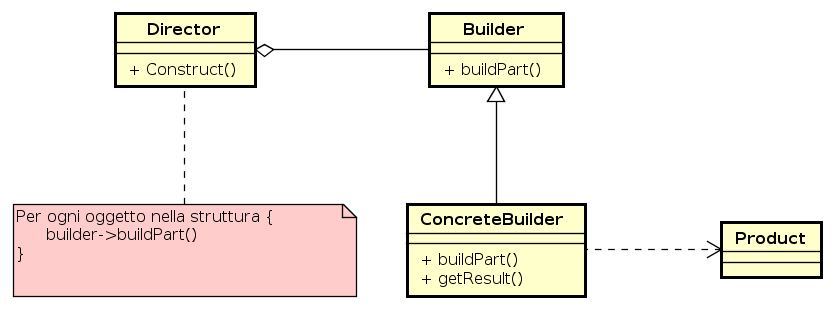
\includegraphics[width=0.8\textwidth]{res/sections/backend/builder.png}
\caption{Design pattern Builder}
\end{figure}
\paragraph{Contestualizzazione}\mbox{} \\
Questo pattern è utilizzato nell'editor nel \glossaryItem{package} \texttt{DSLCreator} per la costruzione di un \glossaryItem{DSL} Element, che in generale può essere un oggetto complesso costituito da più parti. È possibile costruire separatamente le diverse parti che compongono il \glossaryItem{DSL} Element. \\ L'interfaccia \texttt{DSLCreator::Builder} è la base da cui derivano tutte le classi Builder concrete (una per ciascun tipo di \glossaryItem{DSL} Element).
\begin{figure}[H]
\centering
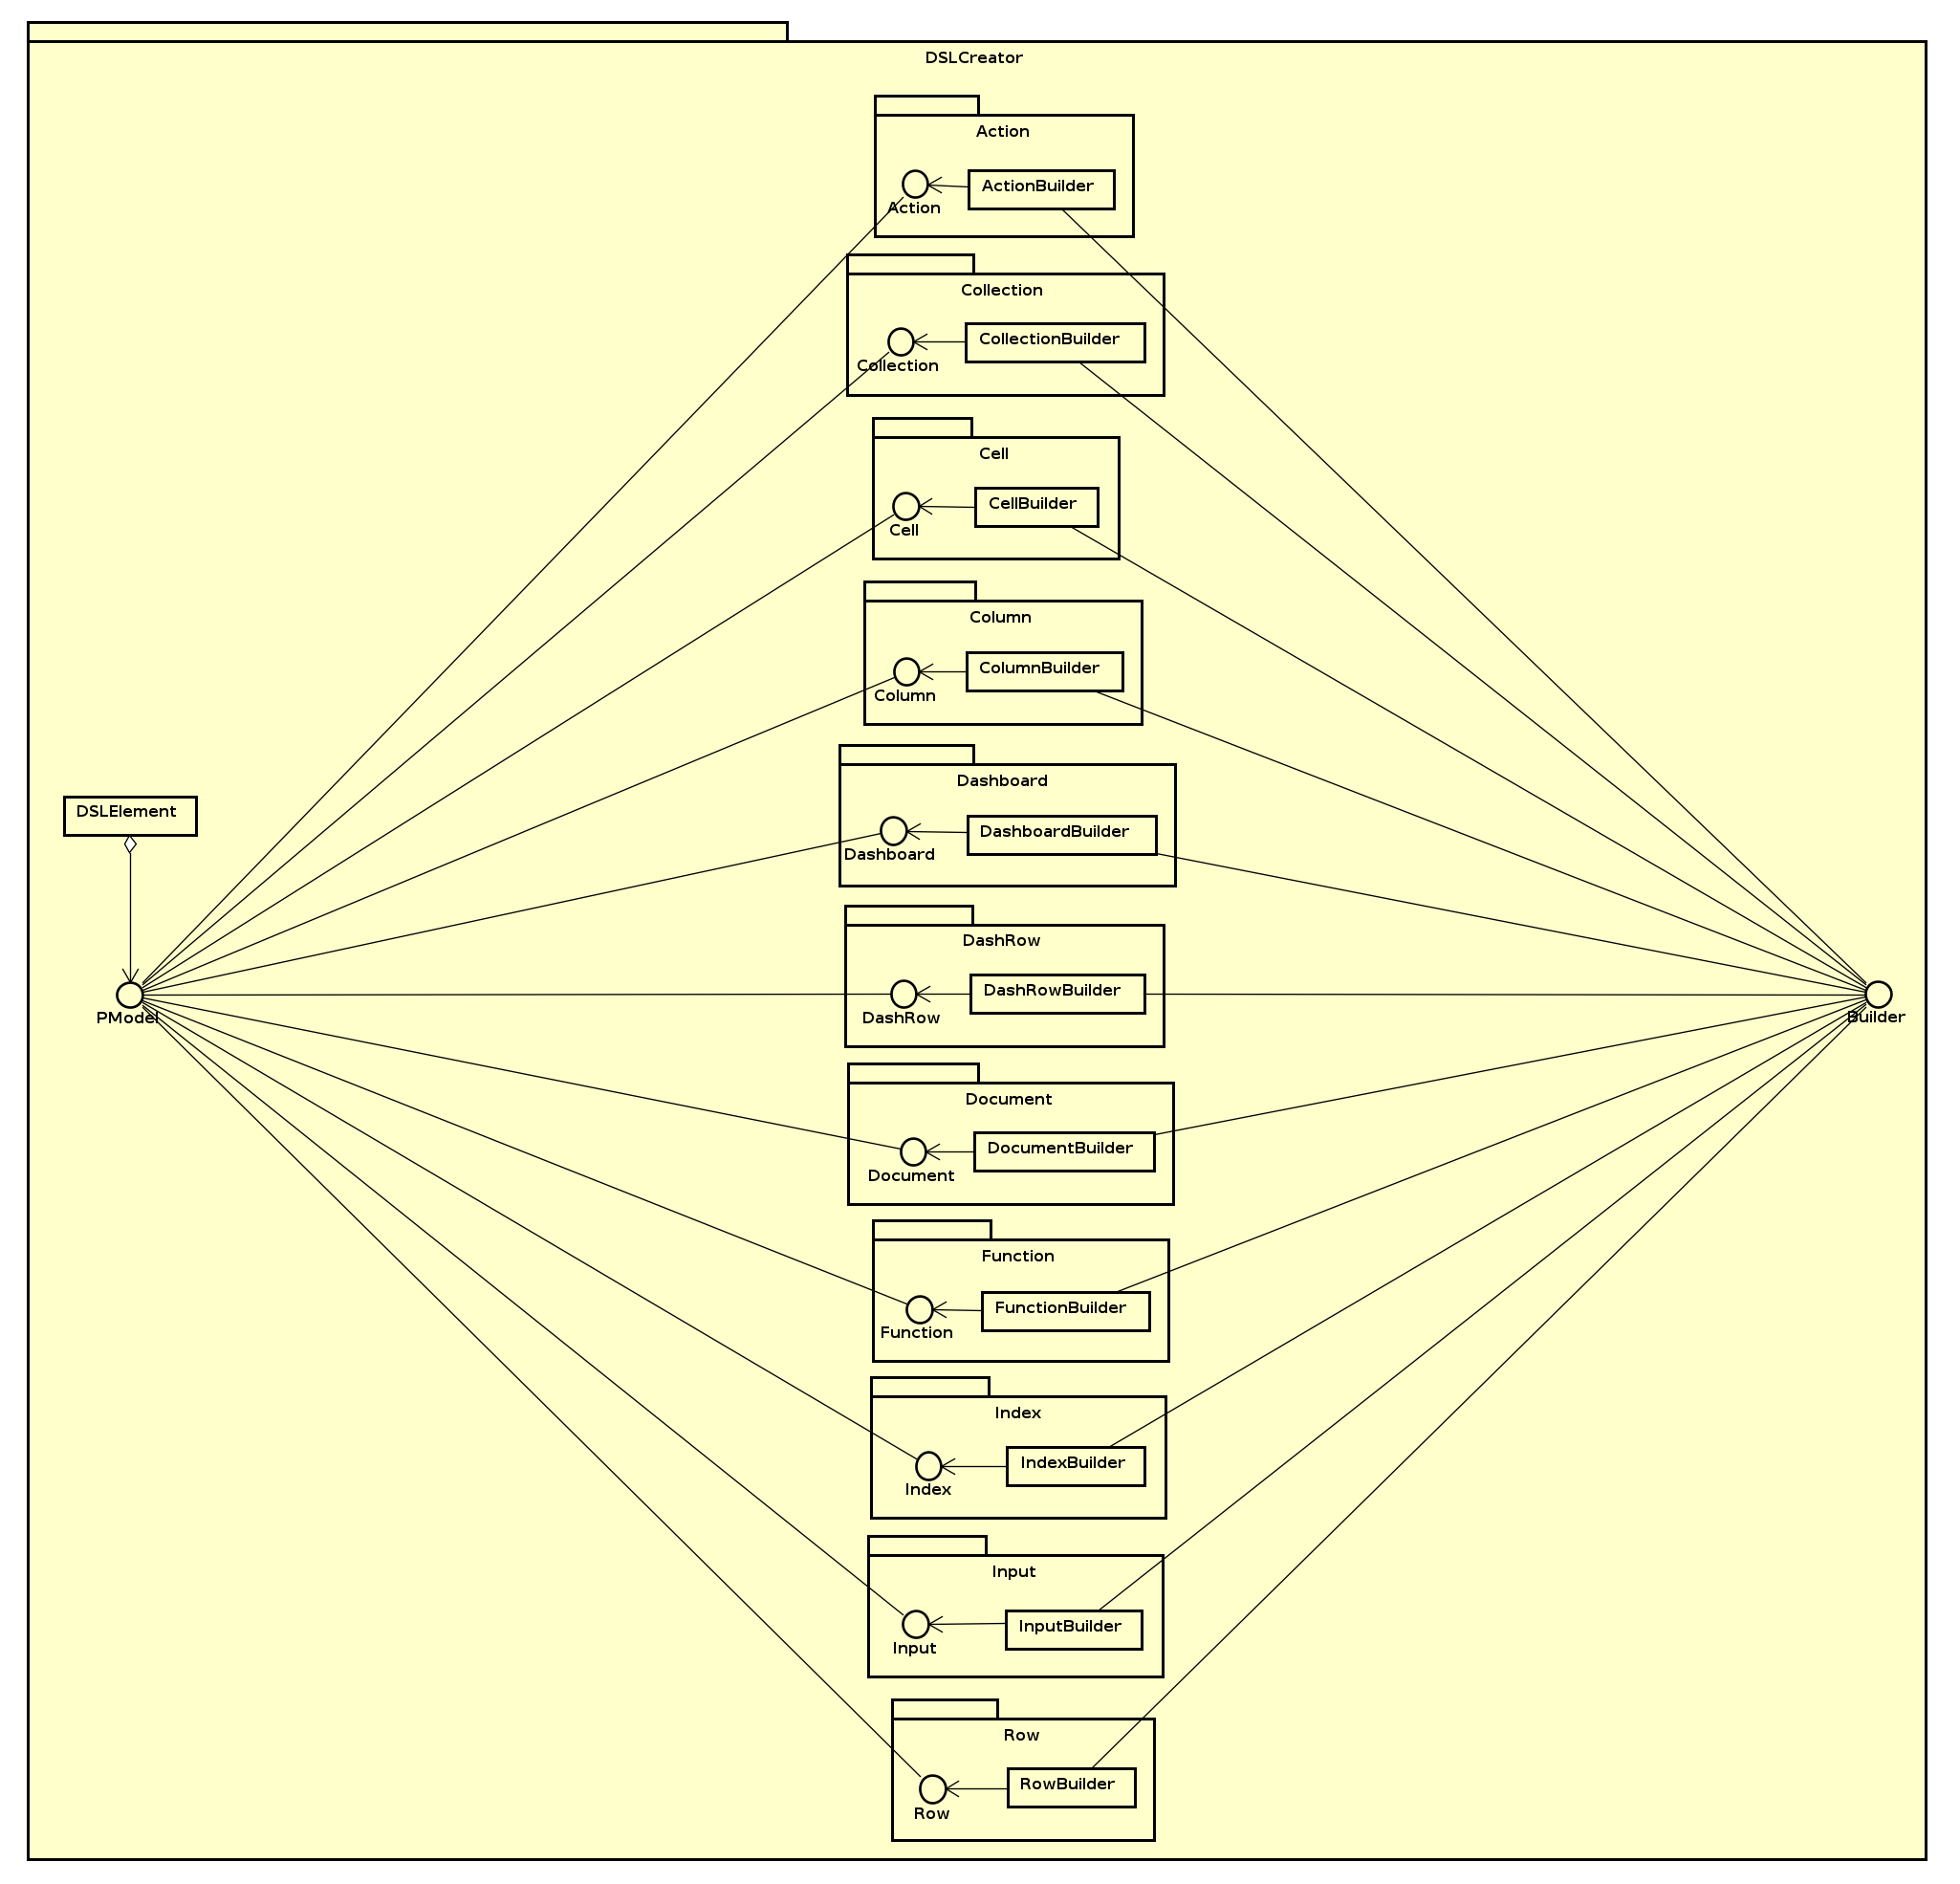
\includegraphics[width=1.0\textwidth]{res/sections/frontend/builder_editor.png}
\caption{Builder nell'editor}
\end{figure}
\subsubsection{Singleton}
\paragraph{Descrizione} \mbox{} \\
Lo scopo del \textit{design pattern} creazionale denominato \textit{Singleton} è assicurare l’esistenza di un'unica istanza di una classe e fornire un punto di accesso globale ad essa. Questo pattern è nato per rispondere alla necessità di non avere più istanze della stessa classe, anche nei linguaggi in cui non è possibile usare una variabile globale, pur dando la possibilità alla classe di tener traccia di quella sua istanza. Il \textit{Singleton} è quindi applicabile ogniqualvolta debba esistere una sola istanza di una certa classe in tutta l’applicazione, prestando però attenzione al fatto che l’istanza sia estendibile tramite ereditarietà.
\paragraph{Vantaggi} \mbox{} \\
\begin{itemize}
\item Controllo completo di come e quando i client accedono all’interfaccia della classe;
\item Evita l’utilizzo ingiustificato di variabili globali;
\item Consente di ridefinire le operazioni definite nel \textit{Singleton};
\item Permette di porre un limite massimo al numero di istanze di una certa classe.
\end{itemize}
\paragraph{Svantaggi} \mbox{} \\
\begin{itemize}
\item Può essere usato male e solo per modellare una variabile globale;
\item Viola il \textit{Single Responsibility Principle}: controlla sia la propria creazione sia il proprio ciclo di vita.
\end{itemize}
\paragraph{Struttura} \mbox{} \\
\begin{figure}[H]
\centering
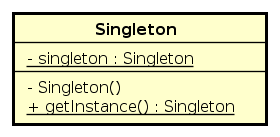
\includegraphics[width=0.5\textwidth]{res/sections/backend/singleton.png}
\caption{Design pattern Singleton}
\end{figure}
\paragraph{Contestualizzazione}\mbox{} \\
Questo pattern viene utilizzato nell'editor nel \glossaryItem{package} \texttt{DSLCreator}, per assicurare che esista una sola istanza della classe \texttt{DSLCreator::Facade}.
\begin{figure}[H]
\centering
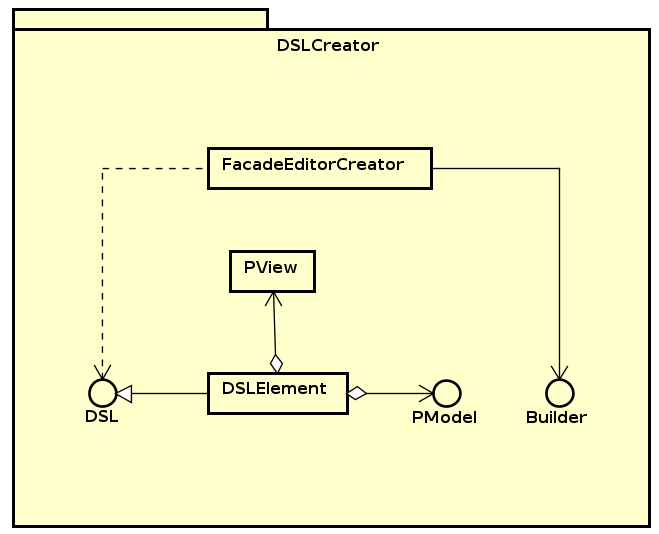
\includegraphics[width=0.9\textwidth]{res/sections/frontend/facade_editor.png}
\caption{Singleton e facade nell'editor}
\label{fig:singleton_editor}
\end{figure}
\subsection{Strutturali}
\subsubsection{Facade}
\paragraph{Descrizione} \mbox{} \\
Questo \textit{design pattern} fornisce un'interfaccia unificata per un insieme di interfacce presenti in un sottosistema. Facade definisce un'interfaccia di alto livello che rende il sottosistema più semplice da utilizzare. Suddividere un sistema in sottosistemi aiuta a ridurne la complessità. Il suo scopo è rendere una libreria più facile da usare, capire, testare e leggere, riducendo al contempo le dipendenze da codice esterno per le operazioni interne. Di solito si usa quando:
\begin{itemize}
\item un'interfaccia semplice deve accedere ad un sistema complesso;
\item l'astrazione e l'implementazione sono molto accoppiate;
\item si necessita di un punto di entrata per ogni livello di un software a strati;
\item un sistema è molto complesso e difficile da capire.
\end{itemize}
\paragraph{Vantaggi} \mbox{} \\
\begin{itemize}
\item Disaccoppia il sottosistema dai client e dagli altri sottosistemi, promuovendo quindi la portabilità e l'indipendenza di sottosistemi;
\item Permette di organizzare i sottosistemi in una struttura a livelli;
\item Fornisce una vista semplice di base su un sottosistema che si rivela essere sufficiente per la maggior parte dei client.
\end{itemize}
\paragraph{Svantaggi} \mbox{} \\
\begin{itemize}
\item Non aggiunge funzionalità, semplifica solamente le interfacce;
\item Non nasconde completamente le componenti di un sottosistema;
\item È un \textit{Single point of failure}, ovvero se non funziona la classe Facade il problema si diffonde sul resto.
\end{itemize}
\paragraph{Struttura} \mbox{} \\
\begin{figure}[H]
\centering
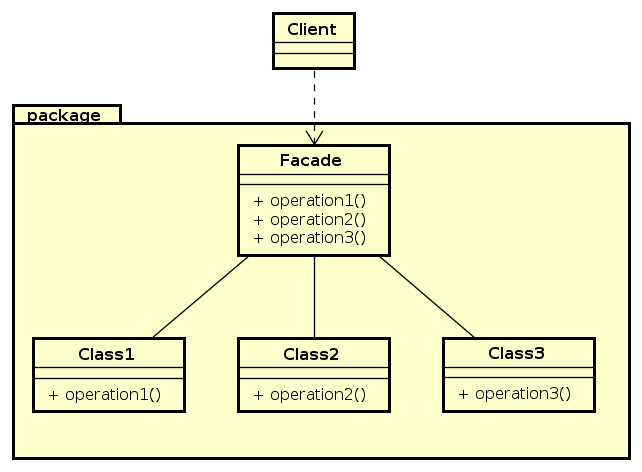
\includegraphics[width=0.8\textwidth]{res/sections/backend/facade.png}
\caption{Design pattern Facade}
\end{figure}
\paragraph{Contestualizzazione}\mbox{} \\
Il \textit{design pattern} \textit{Facade} è utilizzato nel backend per fornire un'interfaccia semplice per il sottosistema complesso del \glossaryItem{package} \texttt{Routes}. Un \glossaryItem{modulo}, FacadeRouter, fornisce l'interfaccia, ed evita a MaaSServer di dover interagire con i singoli \glossaryItem{moduli} rappresentanti le diverse \textit{Routes}. \\
Di seguito è riportato il \glossaryItem{diagramma delle classi} che realizza il \textit{design pattern} \textit{Facade} nel backend.
\begin{figure}[H]
\centering
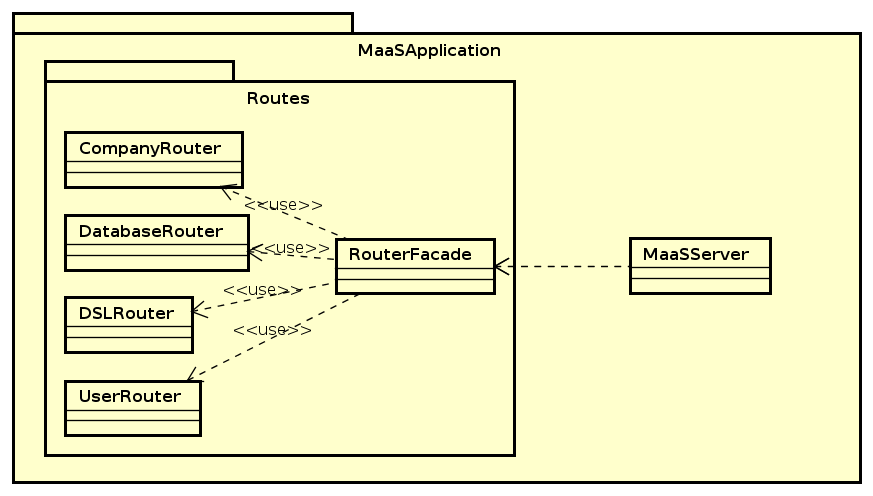
\includegraphics[width=0.8\textwidth]{res/sections/backend/facadeRoutes.png}
\caption{Design pattern Facade nel backend}
\end{figure}
Questo pattern viene utilizzato anche nel frontend, nel \glossaryItem{package} \texttt{DSLCreator}. La classe \texttt{DSLCreator::FacadeEditorCreator} è la classe che espone le funzionalità di creazione di un \glossaryItem{DSL} Element. Al suo interno utilizza la classe \texttt{DSLCreator::Builder} ed usa il \textit{Builder Pattern}. Tale classe è un \textit{Singleton}. (vedi figura \ref{fig:singleton_editor})
\subsection{Comportamentali}
\subsubsection{Chain of responsibility}
\paragraph{Descrizione} \mbox{} \\
Il \textit{Chain of Responsibility} permette di separare i \textit{sender} dai \textit{receiver} delle richieste. La richiesta attraversa una catena di oggetti per essere intercettata solo quando raggiunge il proprio gestore. Viene utilizzato quando non è possibile determinare staticamente il \textit{receiver} oppure l’insieme di oggetti gestori cambia dinamicamente a \textit{runtime}. \\
Le richieste vengono dette implicite poiché il \textit{sender} non ha alcuna conoscenza sull’identità del ricevente. Per permettere alla richiesta di attraversare la catena e per rimanere implicita, ogni \textit{receiver} condivide un interfaccia comune per gestire le richieste ed accedere al proprio successore. La gerarchia che vorrà inviare richieste dovrà avere una superclasse che dichiara un metodo \textit{handler} generico.
\paragraph{Vantaggi} \mbox{} \\
\begin{itemize}
\item Porta ad un accoppiamento debole tra i componenti;
\item Aggiunge flessibilità nell’assegnamento delle responsabilità degli oggetti.
\end{itemize}
\paragraph{Svantaggi} \mbox{} \\
\begin{itemize}
\item Non c’è garanzia che la \textit{request} venga gestita: questo può avvenire quando la catena non è stata costruita in modo rigoroso.
\end{itemize}
\paragraph{Struttura} \mbox{} \\
\begin{figure}[H]
\centering
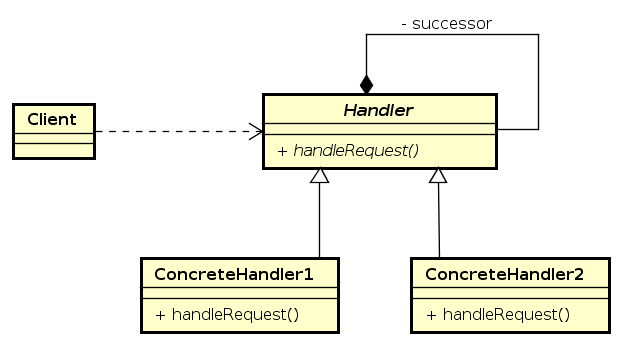
\includegraphics[width=0.8\textwidth]{res/sections/backend/chainOfResponsability.png}
\caption{Design pattern Chain of responsibility}
\end{figure}
\paragraph{Contestualizzazione}\mbox{} \\
La classe \texttt{DSLInterpreter::DSLInterpreter} implementa il \textit{Chain of Responsibility} e detiene una lista di tutti gli interpreti (i \textit{receiver}) da invocare man mano che vengono applicate le traduzioni (le richieste dei \textit{sender}). Il risultato di ogni interprete verrà concatenato e come risultato si otterrà la specifica \glossaryItem{DSL} richiesta.
\begin{figure}[H]
\centering
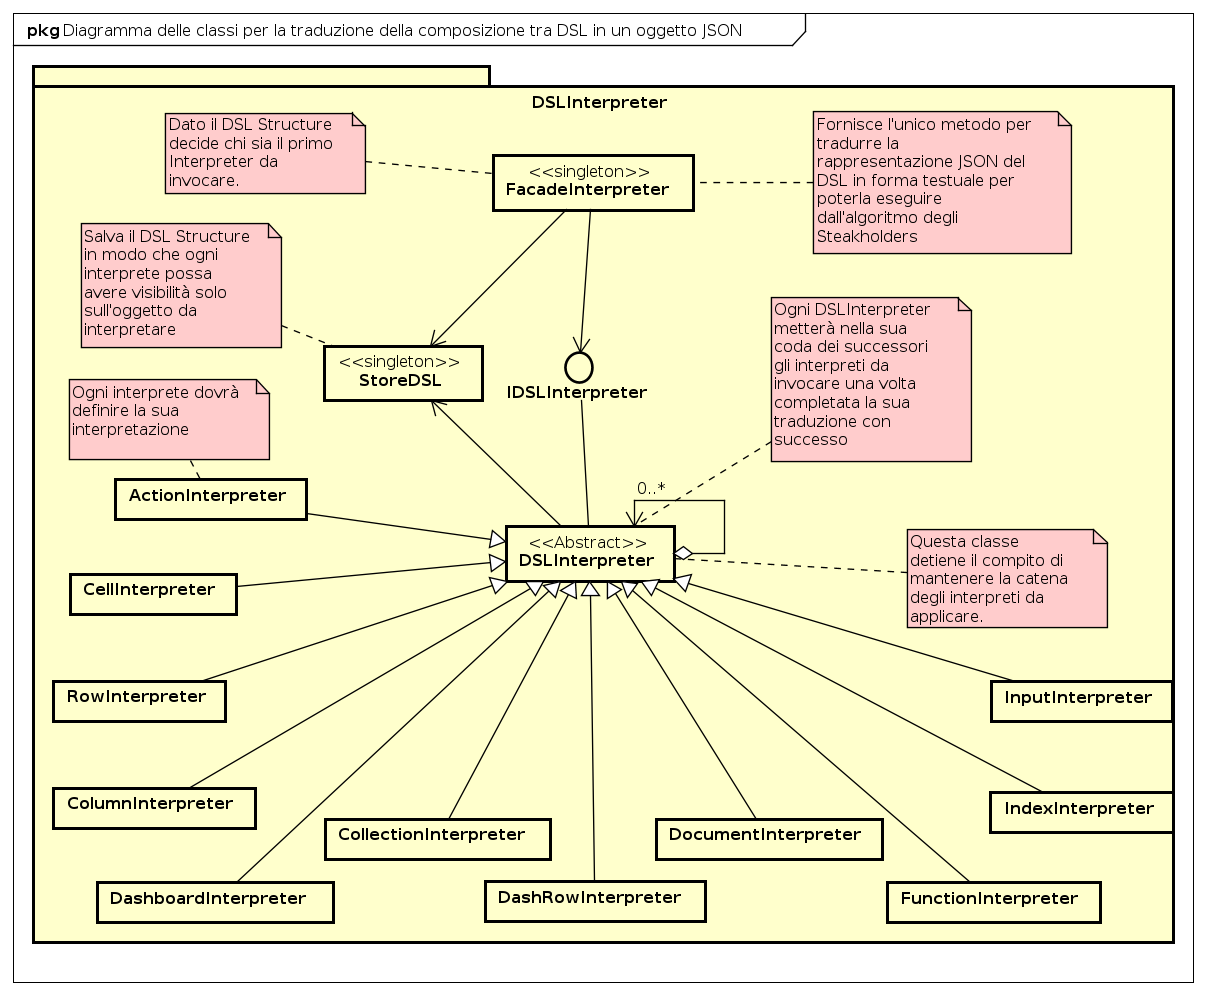
\includegraphics[width=0.9\textwidth]{res/sections/frontend/chainOfResponsability.png}
\caption{Design pattern Chain of responsability nel frontend}
\end{figure}
\subsection{Architetturali}
\subsubsection{Model-View-Controller}
\paragraph{Descrizione} \mbox{} \\
Il pattern è basato sulla separazione dei compiti fra i componenti software che interpretano tre ruoli principali:
\begin{itemize}
\item il \textbf{Model} fornisce i metodi per accedere ai dati utili all'applicazione;
\item il \textbf{View} visualizza i dati contenuti nel \textbf{Model} e si occupa dell'interazione con utenti e agenti;
\item il \textbf{Controller} riceve i comandi dell'utente (in genere attraverso il \textbf{View}) e li attua modificando lo stato degli altri due componenti.
\end{itemize}
Questo schema, fra l'altro, implica anche la tradizionale separazione fra la logica applicativa (in questo contesto spesso chiamata \textit{business logic}), a carico del \textbf{Controller} e del \textbf{Model}, e l'interfaccia utente a carico del \textbf{View}. \\
Quasi sempre la relazione fra \textbf{View} e \textbf{Model} è descrivibile anche come istanza del pattern \textit{Observer}. A volte, quando è necessario cambiare il comportamento standard dell'applicazione a seconda delle circostanze, il \textbf{Controller} implementa anche il pattern \textit{Strategy}.
\paragraph{Vantaggi} \mbox{} \\
\begin{itemize}
\item \glossaryItem{Riuso} dei componenti dei model: miglior manutenzione e test;
\item Supporto più semplice per nuovi tipi di client: basta creare un nuovo \textbf{View} e un nuovo \textbf{Controller}.
\end{itemize}
\paragraph{Svantaggi} \mbox{} \\
\begin{itemize}
\item Maggiore complessità di progettazione: c'è bisogno di molte più classi per garantire la separazione.
\end{itemize}
\paragraph{Struttura} \mbox{} \\
Il seguente diagramma, non \glossaryItem{UML}, mostra la struttura generale del design pattern MVC.
\begin{figure}[H]
\centering
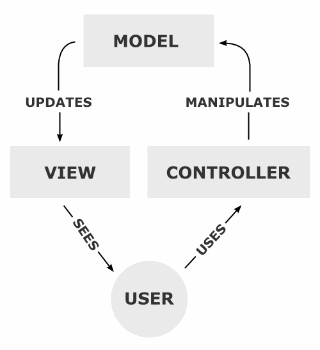
\includegraphics[height=5cm]{res/sections/backend/mvc.png}
\caption{Design pattern Model-View-Controller}
\end{figure}
\paragraph{Contestualizzazione} \mbox{} \\
In \glossaryItem{MaaS}, i componenti che realizzano il design pattern MVC sono i seguenti:
\begin{itemize}
\item \glossaryItem{Package} \texttt{Models} -> \textbf{Model};
\item \glossaryItem{Package} \texttt{Routes} -> \textbf{Controller};
\item Viste di \texttt{React.js} -> \textbf{View}.
\end{itemize}
L'utente interagisce con le viste create tramite il \glossaryItem{framework} React.js. I dati vengono richiesti al server attraverso le \glossaryItem{API} \glossaryItem{REST} messe a disposizione. Le richieste vengono gestite con le routes di ExpressJS, e i \glossaryItem{moduli} del \glossaryItem{package} Models vengono utilizzati per accedere ai dati memorizzati dall'applicazione.
